\documentclass[12pt]{book}
\usepackage[a4paper, total={6in, 8in}]{geometry}
\usepackage{amssymb}
\usepackage{listings}
\usepackage{color}
\usepackage{graphicx}
\usepackage{subfig}
\usepackage{float}
\definecolor{mygrey}{gray}{.96} % Light Grey
\definecolor{BrickRed}{RGB}{120,0,0}


\def\xbf{\mathbf{x}}
\def\zbf{\mathbf{z}}
\def\xibf{\mathbf{\xi}}
\lstset{
	language=C++,              % choose the language of the code ("language=Verilog" is popular as well)
   tabsize=3,							  % sets the size of the tabs in spaces (1 Tab is replaced with 3 spaces)
	basicstyle=\footnotesize,               % the size of the fonts that are used for the code
	numbers=left,                   % where to put the line-numbers
	numberstyle=\footnotesize,              % the size of the fonts that are used for the line-numbers
	stepnumber=1,                   % the step between two line-numbers. If it's 1 each line will be numbered
	numbersep=5pt,                  % how far the line-numbers are from the code
	backgroundcolor=\color{mygrey}, % choose the background color. You must add \usepackage{color}
	showspaces=false,              % show spaces adding particular underscores
	showstringspaces=false,        % underline spaces within strings
	showtabs=false,                % show tabs within strings adding particular underscores
	frame=single,	                 % adds a frame around the code
	tabsize=3,	                    % sets default tabsize to 2 spaces
	captionpos=b,                   % sets the caption-position to bottom
	breaklines=true,                % sets automatic line breaking
	breakatwhitespace=false,        % sets if automatic breaks should only happen at whitespace
	%escapeinside={\%*}{*)},        % if you want to add a comment within your code
	commentstyle=\color{BrickRed}   % sets the comment style
}

\begin{document}
\title{\textbf{Monte Carlo Simulation Lab}}	
\title{\textbf{Assignment-3}}
\author{Yash Vanjani\\(140123046)\\Mathematics and Computing\\IIT Guwahati}
\date{February 9th, 2016}

\maketitle

\newpage
\begin{enumerate}
\item[Q 1] Simulate $5000$ sample of exponential with mean $5$. Draw the histogram and the calculate the mean, maximum and minimum
\end{enumerate}
\noindent{Code for C++}

\begin{lstlisting}
#include <iostream>
#include <cmath>
#include <fstream>

using namespace std;

int main()
{
	ofstream myfile;
	myfile.open("output.txt");
	int a=167, b= 59, x=23, e;
	int m=pow(2,15);
	double E[5000]={0};
	double u, sum=0;
	int freq[35]={0};
	int i;
	for(i=0;i<5000;i++)
	{
		x=(a*x+b)%m;
		u=double(x)/double(m);

		if(u<0.0001)
		{
			i--;
		}
		else
		{
			E[i]=-5*log(u);
			e=int(E[i]);
			freq[e]++;
		}
	}
	for(i=0;i<35;i++)
		myfile<<"freq["<<i<<"]="<<freq[i]<<"\n";

	double max=E[0], min=E[0];
	for(i=0;i<5000;i++)
	{
		if(E[i]>max)
			max=E[i];
		if(E[i]<min)
			min=E[i];
		sum=sum+E[i];
	}
	double mean=double(sum)/5000;
	myfile<<"\nmean = "<<mean<<"\n";
	myfile<<"max = "<<max<<"\n";
	myfile<<"min = "<<min<<"\n";

	myfile.close();
}
\end{lstlisting}
The output of the code is as follows:\\\\
\begin{lstlisting}
freq[0]=934
freq[1]=729
freq[2]=587
freq[3]=485
freq[4]=402
freq[5]=340
freq[6]=267
freq[7]=243
freq[8]=181
freq[9]=149
freq[10]=130
freq[11]=102
freq[12]=86
freq[13]=65
freq[14]=57
freq[15]=45
freq[16]=33
freq[17]=30
freq[18]=23
freq[19]=20
freq[20]=13
freq[21]=14
freq[22]=10
freq[23]=10
freq[24]=9
freq[25]=5
freq[26]=6
freq[27]=5
freq[28]=4
freq[29]=4
freq[30]=3
freq[31]=2
freq[32]=0
freq[33]=1
freq[34]=1

mean = 5.00691
max = 45.0546
min = 0.00015259
\end{lstlisting}
The code in R is shown below:\\
\begin{lstlisting}
m<-2^15
a<-167
b<-59
x<-23
E<-array(0,5000)
freq<-array(0,35)
for(i in 1:5000)
{
	x<-(a*x+b)%%m
	u<-as.double(x)/m
	if(u<0.0001)
	{
		i<-i-1;
	}
	else
	{
		E[i]<- -5*log(u)
		e<- as.integer(E[i])
		freq[e]=freq[e]+1
	}
}
mean=mean(E)
min=min(E)
max=max(E)
cat("Max is:",max,"\n")
cat("min is:",min,"\n")
cat("mean is:",mean,"\n")
barplot(freq,main="X ~ Exp(1/5)", xlab="X",ylab="Frequency",xlim=c(0,40),ylim=c(0,800),col=c("darkblue"));
\end{lstlisting}
The output of the R is shown below:\\
\begin{lstlisting}
Max is: 45.05457 
Min is: 0.0001525902 
Mean is: 5.006914 

\end{lstlisting}
\newpage
The histogram is shown below:
\begin{figure}[H]
	\centering
	\subfloat[$X \sim Exp(1/5)$]{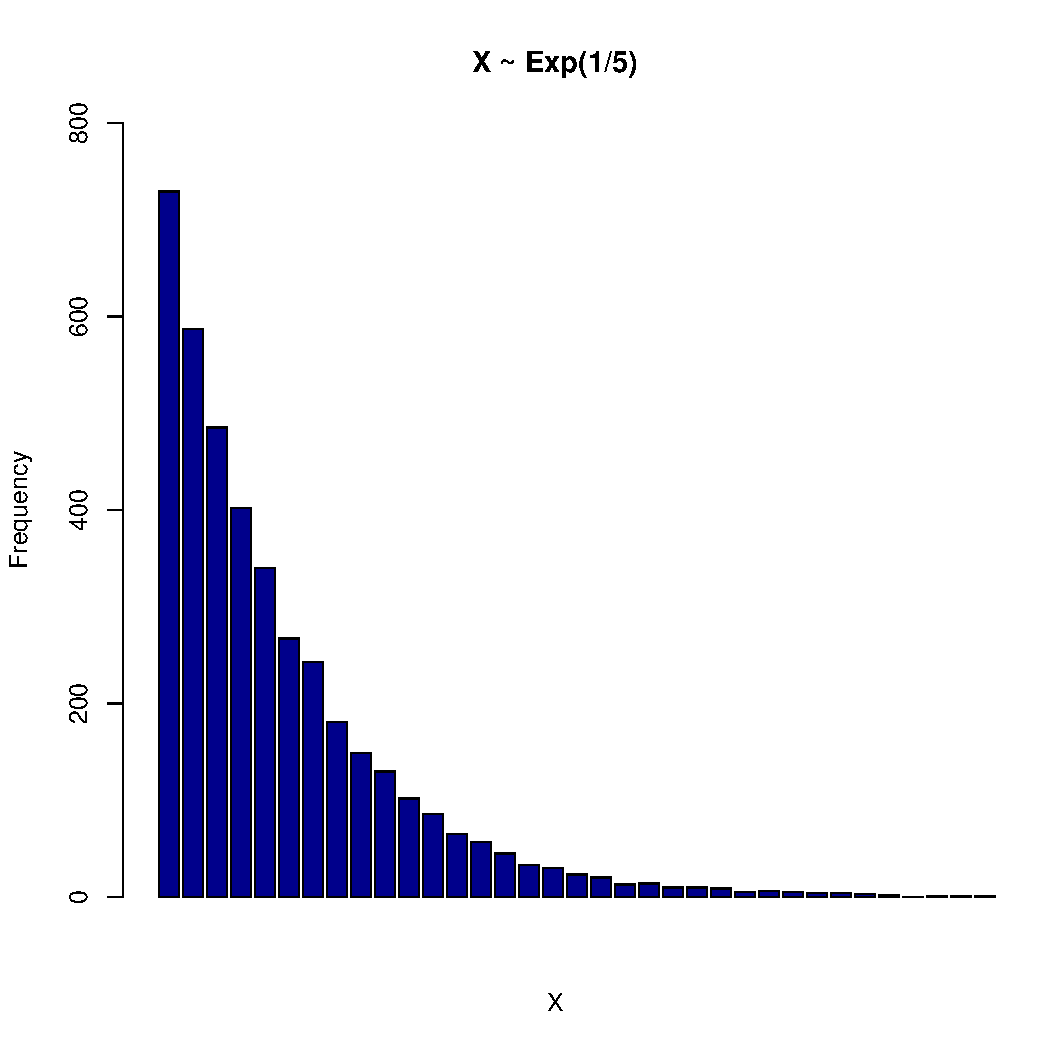
\includegraphics[width=1.0\textwidth]{assign3_q1.pdf}}	
\end{figure}
\newpage

\begin{enumerate}
\item[Q 2] Simulate $5000$ sample of Gamma with parameter $n=5$ and $\lambda=5$. Draw the histogram and the calculate the mean, maximum and minimum.
\end{enumerate}
\noindent{Code for C++}

\begin{lstlisting}
#include <iostream>
#include <cmath>
#include <fstream>
#include <cstdio>


using namespace std;

int main()
{
	ofstream myfile;
	int m[5]={(int)pow(2,17),(int)pow(2,19),(int)pow(2,23),(int)pow(2,27),(int)pow(2,29)};
	int a[5]={167,93,7,123,135};
	int b[5]={371,33,294,4,357};
	int x[5]={55,29,435,99,123};
	double u[5];
	double E[5000][5]={log(0.5)};
	double G[5000],sum=0;
	int freq[50]={0},e;
	for(int j=0;j<5;j++)
	{
		for(int i=0;i<5000;i++)
		{
			x[j]=(x[j]*a[j]+b[j])%m[j];
			u[j]=(double)x[j]/m[j];
			if(u[j]<0.0001)
				i--;
			else
				E[i][j]=log(u[j]);
		}
	}
	double max=G[0];
	double min=G[0];
	for(int i=0;i<5000;i++)
	{
		G[i]=0;
		for(int j=0;j<5;j++)
			G[i]+=E[i][j];
		G[i]=-0.2*G[i];
		e=(int)(G[i]*10);
		sum+=G[i];
		max=(G[i]>max)?G[i]:max;
		min=(G[i]<min)?G[i]:min;
		freq[e]++;
	}
	myfile.open("output1.txt");
	FILE* fp=fopen("output.txt","w");
	double M=sum/5000;
	myfile<<"Mean of the distribution = "<<M<<endl;
	myfile<<"Min = "<<min<<endl<<"Max = "<<max<<endl;
	for(int i=0;i<30;i++)
		fprintf(fp,"%d\n",freq[i]);
	fclose(fp);
	myfile.close();
}
\end{lstlisting}
The output of the code is as follows:\\\\
\begin{lstlisting}
Mean of the distribution = 0.994363
Min = 0
Max = 5.13151
\end{lstlisting}
The code in R is shown below:\\
\begin{lstlisting}
m<-c(2^17,2^19,2^23,2^27,2^29);
a<-c(167,93,7,123,135);
b<-c(371,33,294,4,357);
x<-c(55,29,435,99,123);
E<-matrix(log(0.5),nrow=5000,ncol=5);
freq<-array(0,50);
u<-array(0,5);
for(j in 1:5)
{
	for(i in 1:5000)
	{
		x[j]<-(a[j]*x[j]+b[j])%%m[j];
		u[j]<-as.double(x[j])/m[j];
		if(u[j]<0.0001)
		{
			i<-i-1;
		}
		else
		{
			E[i,j]<- log(u[j]);
		}
	}
}
G<-array(0,5000);
for(i in 1:5000)
{
	G[i]<-sum(E[i,]);
	G[i]<- -0.2*G[i];
	e<-as.integer(G[i]*10);
	freq[e+1]<-freq[e+1]+1;
}
M<-mean(G);
max<-max(G);
min<-min(G);
cat("Max is:",max,"\n")
cat("min is:",min,"\n")
cat("mean is:",M,"\n")
barplot(freq,main="X ~ Gamma(5,5)", xlab="X",ylab="Frequency",xlim=c(0,40),ylim=c(0,500),col="red");
\end{lstlisting}
The output of the R is shown below:
\begin{lstlisting}
Max is: 3.654517 
Min is: 0.1060267 
Mean is: 0.9912688 
\end{lstlisting}
\newpage
The histogram is shown below:
\begin{figure}[H]
	\centering
	\subfloat[$X \sim Gamma(5, 5)$]{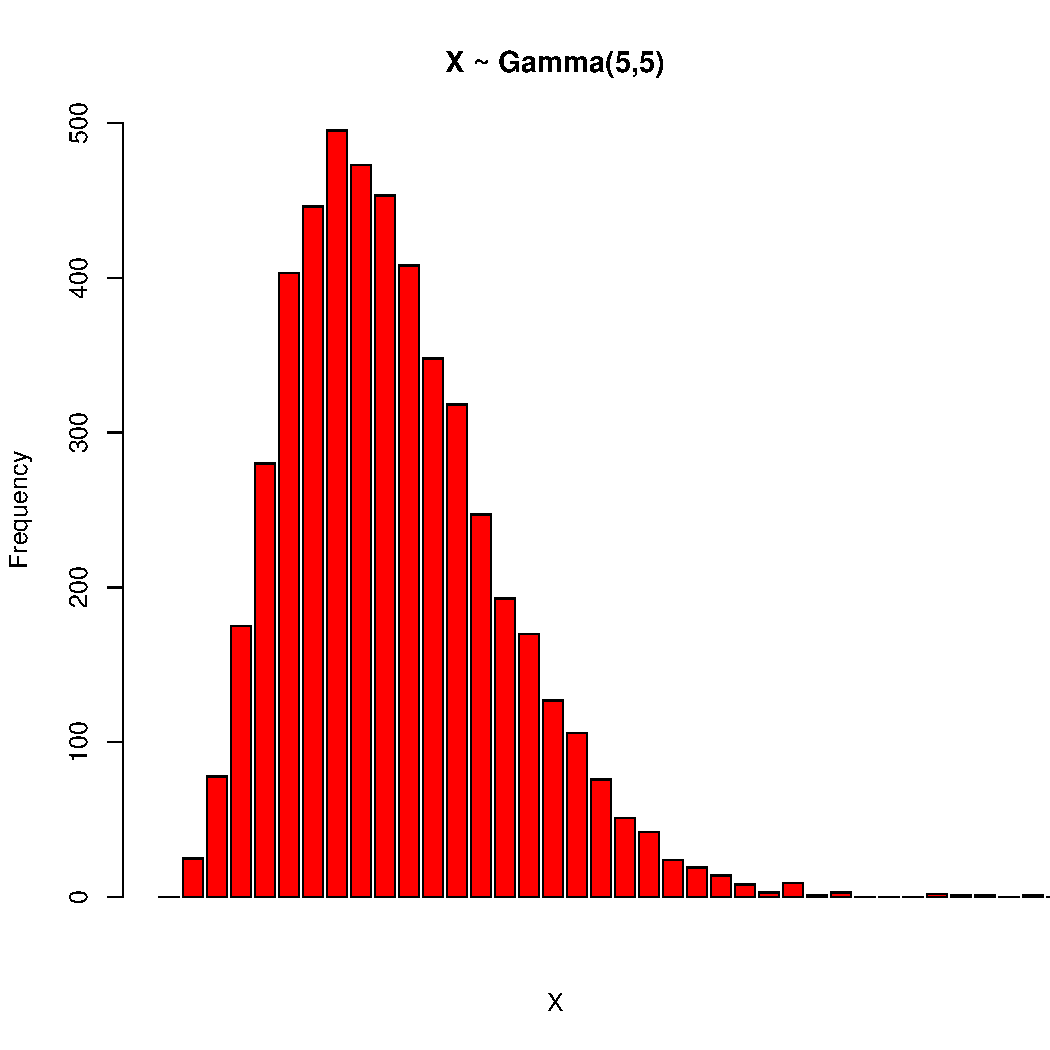
\includegraphics[width=1.0\textwidth]{assign3_q2.pdf}}	
\end{figure}
\newpage
\begin{enumerate}
\item[Q 3] Use the rejection method to generate from $$f(x)=20x(1-x)^3, 0<x<1$$
\end{enumerate}
The code in R is shown below:\\
\begin{lstlisting}
f<-function(x)
{
	return (20*x*(1-x)^3);
}
m<-2^15;
a<-167;
b<-59;
x<-23;
y<-2471;
cg<-2;
freq<-array(0,50);
for(i in 1:50000)
{
	x<-(a*x+b)%%m;
	u<-as.double(x)/m;
	y<-(a*y+b+7)%%m;
	v<-as.double(y)/m;
	if(cg*u<=f(v))
		freq[v*50+1]<-freq[v*50+1]+1;
}
barplot(freq,ylim=c(0,1200),col="green");
\end{lstlisting}
\newpage
The histogram formed is as follows:
\begin{figure}[H]
	\centering
	\subfloat[$f(x)=20x(1-x)^3, 0<x<1$]{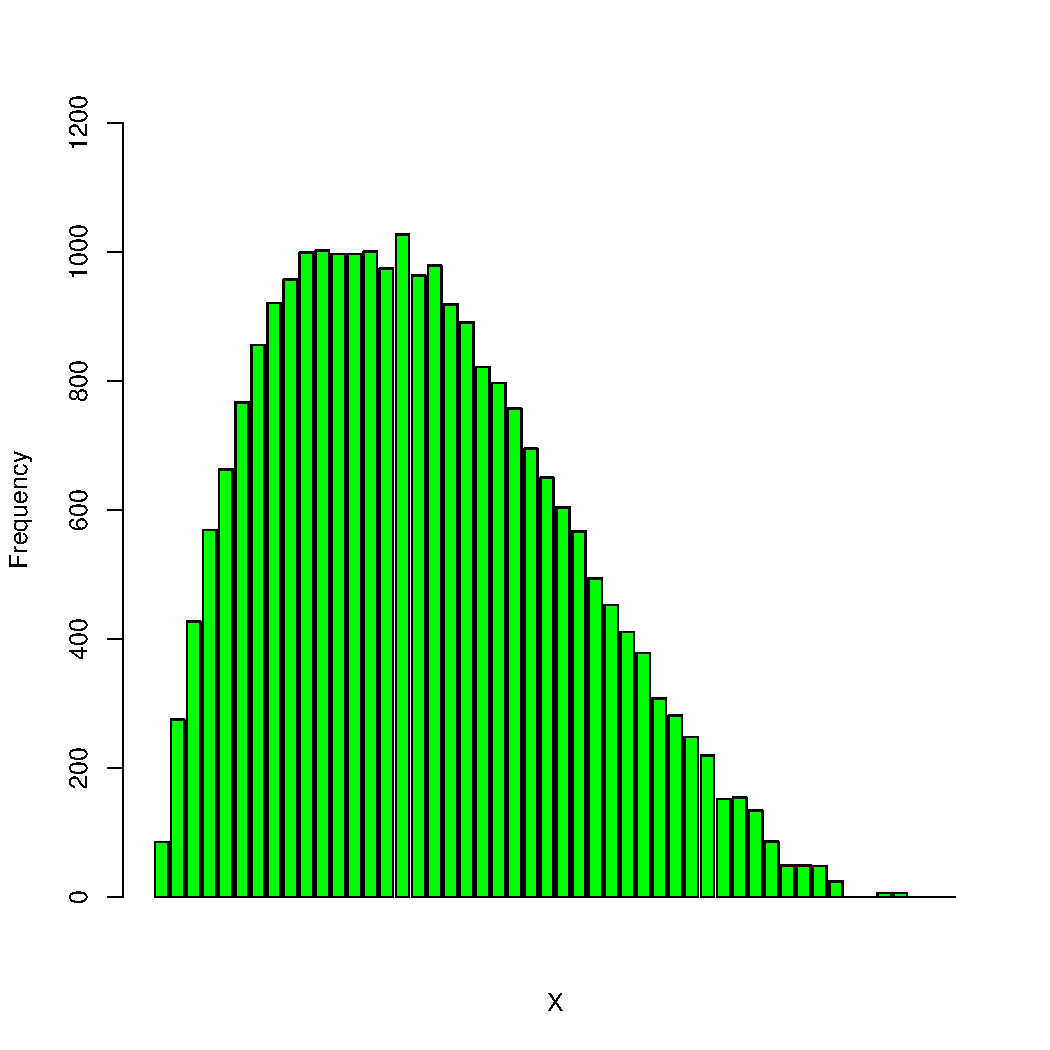
\includegraphics[width=1.0\textwidth]{assign3_q3.pdf}}	
\end{figure}
\end{document}